\chapter{Introduzione}

\section{Il Corso in Breve...}

Questo corso ruota attorno alla parola "\fancyglitter{riduzione}": si evita di reinventare l'acqua calda. La riduzione si collega al concetto di \fancyglitter{intrattabilità}: non si conoscono algoritmi sufficientemente veloci per risolvere un determinato problema per ogni sua istanza (o non esistono ma non lo si sa dimostrare). Il corso è incentrato sulle tecniche per affrontare problemi intrattabili. 

\begin{itemize}
  \item Brute Force.
  \item Backtracking.
  \item Least Cost.
  \item ...
\end{itemize}

\nt{La chiave di lettura per parlare di questi strumenti è proprio la riduzione.}

\subsubsection{}

Successivamente si parlerà di \fancyglitter{correttezza}: dimostrare che un programma restituisca l'output desiderato per qualsiasi istanza di input.

\subsection{Problemi Motivazionali}

\paragraph{Problema delle Valutazioni:} si devono valutare 8 parti di un esame con 50 domande totali per cui si può ottenere un massimo di 125 punti. Il problema consiste nel trovare il modo di massimizzare il voto dato, ma limitandolo a 100 punti.

\qs{}{È facile verificare che l'insieme selezionato è una soluzione? (il voto assegnato è minore o uguale al massimo ammesso)}

\qs{}{È facile verificare che l'insieme selezionato è una risposta? (il voto assegnato premia al massimo l'esaminando)}

\qs{}{È facile scrivere un algoritmo che fornisce una soluzione?}

\qs{}{È facile scrivere un algoritmo che fornisce una risposta?}

\paragraph{Problema del Bando:} l'incubatore dell'azienda TDT bandisce l'assegnazione di 90 unità di denaro per finanziare 3 progetti, uno per ciascuna delle seguenti aree di intervallo:

\begin{itemize}
  \item Area 0. 
  \item Area 1. 
  \item Area 2.
\end{itemize}

\subsubsection{}

I progetti sono classificati in base a un indice di utilità:

\begin{itemize}
  \item Criterio 1. 
  \item Criterio 2. 
  \item ...
\end{itemize}

\nt{Se si decide di finanziare un progetto lo si finanzia per intero.}

\subsubsection{}

\qs{}{È facile certificare un insieme soluzione? (il totale finanziato è minore o uguale 90)}

\qs{}{È facile certificare un insieme risposta? (il totale finanziato è minore o uguale a 90, con utilità massima)}

\qs{}{
  Cosa ha in comune con gli algoritmi sintetizzati per le valutazioni?
}

\paragraph{Problema:} si vuole prestare denaro per un massimo di 220 unità. Il massimo rischio ammissibile è del 40\% (Rischio = $\frac{\text{Richiesta}}{\text{Affidabilità}}$ per singolo finanziamento). Si vuole massimizzare il guadagno. 

\qs{}{È facile verificare che l'insieme selezionato è una soluzione? (il totale finanziamenti è minore o uguale a 220 e il rischio è minore o uguale al 40\%)}

\qs{}{È facile verificare che l'insieme selezionato è una risposta? (il totale finanziamenti è minore o uguale a 220 e il rischio è minore o uguale al 40\%, massimizzando il guadagno)}

\qs{}{Cosa ha in comune con gli algoritmi sintetizzati in precedenza?}

\nt{Questi problemi possono essere ridotti al knapsack.}

\subsection{Strategie di soluzione}

\begin{itemize}
  \item Calcolo classico: soluzione a problemi che coinvolgono funzioni, derivate e integrali. 
\end{itemize}

\paragraph{Dizionario di riferimento (Bellman):}

\begin{itemize}
  \item \fancyglitter{Risorsa economica}: denaro, persone, materiali, etc. disponibile in quantità $x$. 
  \item \fancyglitter{Attività}: modi diversi, da 1 a $N$, in cui possiamo usare la risorsa economica. 
  \item \fancyglitter{Quantità allocate}: $x_1, \dots, x_N$, una per ogni attività.
  \item \fancyglitter{Ricavo singola attività}: $g_i(x_i)$ relativo all'attività $i$. 
  \item \fancyglitter{Ricavo}: valore globale che dipende dal modo in cui ogni attività usa la porzione allocata della risorsa.
\end{itemize}

\ex{Valutazioni}{
\begin{itemize}
  \item \fancyglitter{Risorsa economica}: 100 unità
  \item \fancyglitter{Attività}: 50 correzioni concorrenti. 
  \item \fancyglitter{Quantità allocate}: inclusioni tra risposte per voto.
  \item \fancyglitter{Ricavo singola attività}: voto effettivamente assegnabile da risposta. 
  \item \fancyglitter{Ricavo}: voto finale.
\end{itemize}

}

\nt{Il calcolo classico non è sufficiente a risolvere i problemi motivazionali.}

\qs{}{
  La \fancyglitter{programmazione lineare} (PL) e la \fancyglitter{programmazione lineare intera} (PLI) sono alternative al calcolo classico?
}
\paragraph{La PL non è adatta:} le soluzioni ai problemi Valutazioni, Bando e Rischio assumono la forma di tuple \( x^*_1 , ..., x^*_N \), in cui ogni \( x^*_i \in \{0, 1\} \). In accordo col vocabolario iniziale, questo significa che ogni attività coincide con una scelta:

\begin{itemize}
  \item Se $x^*_i$, l'attività consiste nel \fancyglitter{non scegliere} di inserire il ricavo locale $g_i$ in quello totale. 
  \item Se $x^*_i$, l'attività consiste nel \fancyglitter{scegliere} di inserire il ricavo locale $g_i$ in quello totale.
\end{itemize}
\subsubsection{}
Le tecniche algoritmiche offerte dalla \fancyglitter{PL} sono sviluppate per ottenere valori delle variabili \( x^*_1, \dots, x^*_N \) di problemi esprimibili almeno come:

\begin{equation}
    \max/\min_{\substack{x_1, x_2, \dots, x_N}} \quad g_1(x_1) + g_2(x_2) + \dots + g_N(x_N)
\end{equation}
\[
    \dots
\]
\begin{equation}
    x_i \in \mathbb{R} \quad (i \in \{1, \dots, N\})
\end{equation}
\subsubsection{}
in cui le variabili posso assumere valori in \( \mathbb{R} \). Quindi, non possiamo immaginare di risolvere alcuno dei problemi motivazionali con tecniche di \fancyglitter{PL}.

\paragraph{Anche la PLI può essere inefficiente:} la \fancyglitter{PLI} si distingue dalla PL perché fornisce tecniche per risolvere problemi della forma:

\begin{equation}
    \max/\min_{\substack{x_1, x_2, \dots, x_N}} \quad g_1(x_1) + g_2(x_2) + \dots + g_N(x_N)
\end{equation}
\[
    \dots
\]
\begin{equation}
  x_i \in \{0, 1\} \quad (i \in \{1, \dots, N\})
\end{equation}
\subsubsection{}
in cui le variabili possono assumere valori in $\{0, 1\}$.

\nt{Imponendo variabili discrete, il comportamento della funzione da massimizzare (o minimizzare) diventa non derivabile. Quindi la ricerca dei valori ottimali deve avanzare per tentativi.}

\paragraph{Le euristiche Greedy:}

\begin{itemize}
  \item Allocano una quantità di risorsa per la prossima attività tale da massimizzare il ricavo in quel momento. 
  \item Non ammettono "ripensamenti": non è possibile ritrattare sulla quantità di risorse assegnata a un'attività una volta decisa.
\end{itemize}

\paragraph{Due euristiche Greedy per valutazioni:}

\begin{enumerate}
  \item Si sceglie in base al miglior valore assoluto del voto assegnato. 
  \item Si sceglie in base al miglior rapporto $\frac{\text{voto assegnato}}{\text{voto massimo assegnabile}}$.
\end{enumerate}

  \begin{figure}[h]
    \centering
    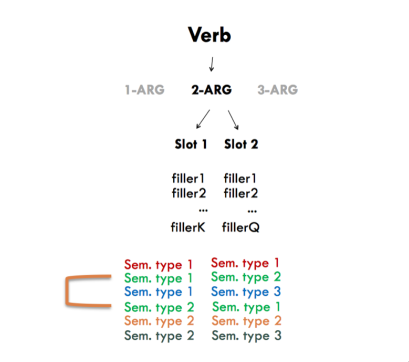
\includegraphics[scale=0.7]{01/val.png}
    \caption{Esempio di valutazioni.}
  \end{figure}

\clm{}{}{
  \begin{itemize}
    \item Se si applica la prima euristica si assegna 7.9 (2+2+3.9). 
    \item Se si applica la seconda euristica si assegna 8.5 (4.6+3.9).
  \end{itemize}

  Però il massimo possibile è 8.6 (2+2+4.6).
}

\nt{Nessuna delle due scelte è ottimale.}

\section{Brute-Force}

Si vuole trovare un algoritmo per risolvere il problema delle valutazioni a \fancyglitter{basso costo computazionale}.

\myalgo{Brute-Force}{
  L'algoritmo Brute-Force effettua una visita esaustiva dello spazio delle permutazioni.
}
  \begin{figure}[h]
    \centering
    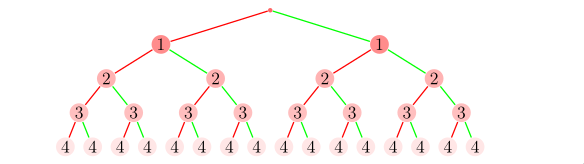
\includegraphics[scale=0.7]{01/bf.png}
    \caption{Applicazione di Brute-Force.}
  \end{figure}
  \nt{Un ramo rosso indica falso (risposta non presa), un ramo verde indica true (risposta presa).}
\clm{}{}{
  \begin{itemize}
    \item La strategia Brute-Force su permutazioni è completa: indivisua \textit{almeno} una risposta che corrisponde alla soluzione migliore. 
    \item Le euristiche Greedy non sono complete.
    \item Con la generazione di permutazioni si può, senza cambiare nulla, avere la soluzione per il problema dei bandi.
  \end{itemize}
}

\subsection{Permutazioni, Disposizioni e Sottoinsiemi}






